\documentclass[11pt, a4paper, draft]{article}
\usepackage{tmh}
\usepackage{bbm}
\renewcommand{\labelenumi}{\roman{enumi})}
\renewcommand{\phi}{\varphi}

\renewcommand{\P}{\mathbb{P}}
\newcommand{\E}{\mathbb{E}}
\renewcommand{\R}{\mathbb{R}}
\newcommand{\T}{\mathbb{T}}
\newcommand{\Z}{\mathbb{Z}}
\newcommand{\F}{\mathcal{F}}
\newcommand{\Dt}{\Delta t}
\newcommand{\Dv}{\Delta v}
\newcommand{\Dx}{\Delta x}
\newcommand{\dx}{\dif x}
\newcommand{\dt}{\dif t}
\renewcommand{\familydefault}{\sfdefault}
\usepackage[scaled]{helvet}
\setlength{\parindent}{0em}
\setlength{\parskip}{1em}

\usepackage{showkeys}

\title{{\huge Interacting Particle Systems} \\\vspace{1cm} Subtitle}
\author{Thomas M. Hodgson\\ \vspace{0.5cm} Maxwell Institute}
\date{\today}

\begin{document}

	\section{Numerical Methods}\label{sec:numericalmethods}
        The analysis presented so far has been able to fully characterise the behaviour of the space-homogeneous kinetic model. However, it is unable to describe the dynamics of the full space-inhomogeneous model. It has been shown that the space-homogeneous model possesses only three invariant measures and converges to one of them dependent on the sign of the mean of the initial data. The full model also has these invariant measures, however it is not proven whether these are all of them or not. That is, the full model may have stationary distributions which are not homogeneous in space. By utilising numerical methods, we can relax some of the restrictions which the analysis requires. The goal is to show that for some choice of initial data and interaction function, the particle system will have a stationary distribution that isn't uniform in space. At its most basic, this could be two clusters of particles moving on the same direction diametrically opposite each other. The system will still converge in velocity to the values predicted by the homogeneous model, but spatial heterogeneity will remain. While this may be the case for the particle system, we conjecture that such behaviour will not occur in the kinetic model.
        
        The aim is to be able to accurately simulate the dynamics of both the space-inhomogeneous PDE +++ref+++ and the corresponding interacting particle system. The latter is relatively simple to simulate using techniques for SDEs. However, we have shown analytically that the particle system does not have the same invariant measures as the continuum model, or indeed its McKean-Vlasov equation. The kinetic model is more difficult as it contains both advective and diffusive terms. We begin this section with a presentation of numerical methods for SDEs before reviewing methods for advection-type and diffusion-type equations, following the treatment of Hundsdorfer and Verwer \cite{Hundsdorfer2007} as well as Morton and Meyers \cite{Morton2005}.
        
        Mirroring the approach in the analysis, we will develop the techniques required first for the space-homogeneous system with no interaction, before adding further levels of complexity. Doing so allows the rigorous testing of any schemes developed as analytic solutions are available.
        
        \subsection{Particle Systems}
        Simulating particle systems requires the numerical solution of coupled SDEs. The standard method for this is the Euler-Maruyama (EM) method, which can be seen as the stochastic analogue of Euler's method. Our motivating example here will be the Ornstein-Uhlenbeck process\footnote{This is also the overdamped Langevin equation}. 
        \begin{equation}
        \dif x^_t = - x_t \dif t + \sigma \dif W_t
        \end{equation}
        This is exactly the same evolution as that which drives the space-homogeneous particle system \eqref{eq:hom_particle}, with no interaction between particles, and so provides the ideal starting point. Applying the EM method to the above equation gives:
        \[ x_{n+1} = x_n -  x_n\Dt + \sqrt{2\sigma\Dt}Z^_n,  \]
        where $Z_n$ is a standard normal random variable. This discretisation is very quick to compute, and has strong order $\frac{1}{2}$ \cite{Higham01}. This gives us a method of finding the stationary distribution: simulate many particles for a long time. Eventually, the density of the particles will be approximately the stationary distribution of the system. In this case it is in fact not even necessary to simulate many particles -- if the system is allowed to evolve for long enough, one particle will suffice as there is no interaction between particles and the scheme is ergodic. The particle system will be an excellent metric by which to test the schemes developed for the continuum models. One drawback however will be the presence of only one invariant measure, as was shown analytically in sec +++ref+++ and will be shown numerically in +++ref+++
        \begin{figure}
            \centering
            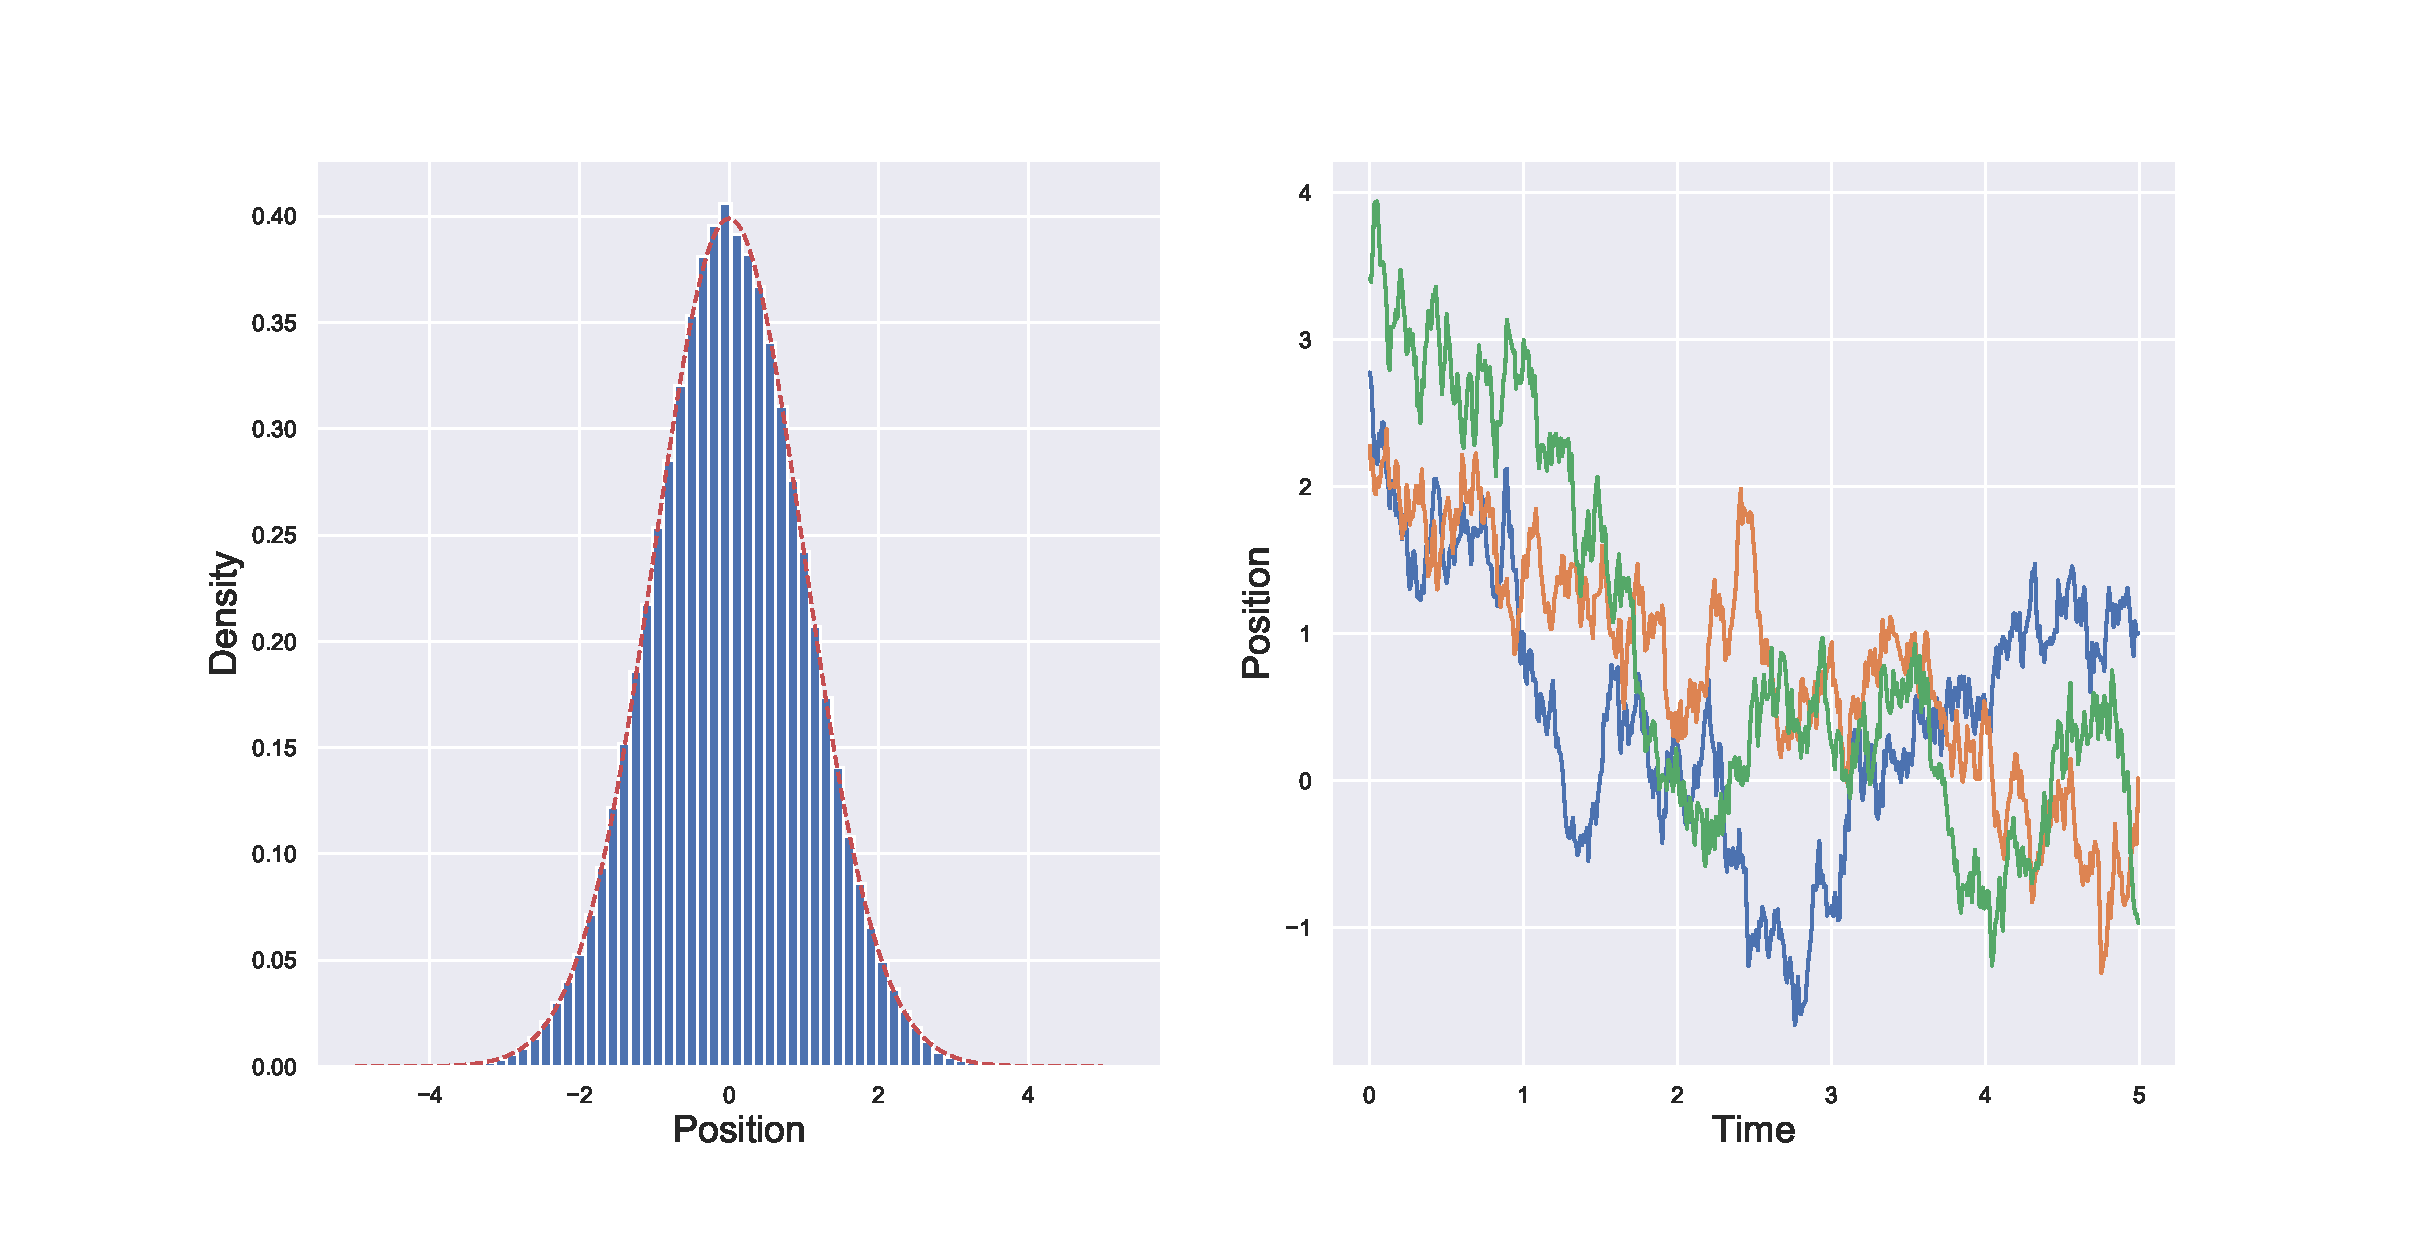
\includegraphics[width=0.7\linewidth]{Figures/OUparticletraj}
            \caption{Histogram of positions of 1000 particles after 100s with $\sigma = 1$, and positions of 5 particles over time.}
            \label{fig:ouparticletraj}
        \end{figure}
        
        \subsection{Diffusion Equations}
        As a prototypical example of a diffusion equation, consider the heat equation in one dimension given by 
        \begin{equation}\begin{cases}
        \partial_t u(t,x) = \sigma\partial_{xx} u(t,x),&\sigma >0\\
        u(0,x) = u_0(x),  &t\in\R^+, x\in\R,
        \end{cases}\label{eq:heat}\end{equation}
        To solve this numerically, we must truncate the domain in both time and space. To do this, a region is chosen where we expect most of the mass to be throughout the time of interest. Here, we truncate to \(x \in [-L,L], t \in [0,T]\) for some \(L>0\) and a finite time horizon \(T\). Doing so requires a boundary condition to be enforced. A natural choice for this equation is a zero Dirichlet condition, \(u(t,L) = u(t,-L) = 0\). As long as \(L\) is chosen large enough, the heat which spreads beyond this limit is negligible. We must also discretise in space and time, to create a mesh covering \(\left[0,T\right] \times \left[-L,L\right]\). Let \(\lbrace x_j\rbrace_{j=0}^J\) partition the space equally such that \(x_0 = -L, x_J=L\) and \(x_j-x_{j-1} = \Delta x\) for all \(j\). Similarly, let \(\lbrace t_n\rbrace_{n=0}^N\) partition \(\left[0,T\right]\) such that \(t_0=0, t_N =T\) and \(t_n-t_{n-1} = \Delta t\). The parameters \(\Delta x, \Delta t\) are the space step and time step respectively. We thus have a description of the continuum that we can implement. 
        
        +++ Picture of mesh +++
        
        The aim is to solve the equation approximately on this grid. We shall denote approximate solutions by capital letters, that is \(u(x_j,t_n) \approx U_j^n\). How can we approximate the solution? We must approximate each term in the equation separately. First the time derivative, or transient term can be approximated using the definition of the derivative. Recall
        \[
        \od{u}{t} = \lim_{\Delta t \to 0}\frac{u(t+\Dt) - u(t)}{\Dt}.
        \]
        We can approximate the derivative by simply taking \(\Dt\) small. Doing so leads to the forward difference approximation
        \[
        \partial_t u(t_n,x_j) \approx \frac{U^{n+1}_j- U^n_j}{\Dt}.
        \]
        
        Now for the diffusion term, the most obvious approximation is to apply the forward difference scheme twice.
        \begin{align*}
        \partial_{xx} u(t_n,x_j) &\approx \partial_x \left(\frac{U^n_{j+1}- U^n_j}{\Dx}\right)\\
        &=  \left(\frac{\partial_xU^n_{j+1} - \partial_xU^n_j}{\Dx}\right)\\
        &\approx \frac{U^n_{j+1} - 2U^n_{j} + U^n_{j-1}}{(\Dx)^2}
        \end{align*}
        This is sufficient to give a first approximation to \eqref{eq:heat}.
        \begin{align}\label{eq:FTCS_heat}
        \frac{U^{n+1}_j- U^n_j}{\Dt} &= \sigma \frac{U^n_{j+1} - 2U^n_{j} + U^n_{j-1}}{(\Dx)^2}\\
        U^{n+1}_j &= U^n_j +  \frac{\sigma\Dt}{(\Dx)^2}\lbrack U^n_{j+1} - 2U^n_{j} + U^n_{j-1}\rbrack 
        \end{align}
        This is the Forward Time Centred Space (FTCS) method, a fully explicit scheme which means that we can write the next time step solely in terms of known values.
        \subsubsection*{Error and Stability of the Fully Explicit Scheme}
        We now have a method for approximating the true solution, but have not yet considered its accuracy or stability. The heat equation \eqref{eq:heat} can be solved by separation of variables, giving the solution as a Fourier series. If the initial data is a single Fourier mode, the solution is
        \begin{align*}
            &u(t,x) = \mathrm{e}^{-\sigma(2\pi k)^2 t} \phi_k(x), && \phi_k(x) = \mathrm{e}^{2\pi i k x} \text{ for } k \in \Z.
        \end{align*} 
        If we similarly write our approximate solution as a Fourier mode, a criterion for stability will emerge.
        \begin{align*}
            &U^n_j = \lambda^n \mathrm{e}^{ik(j\Dx)}, \qquad k \in \Z \\
            \implies &U^{n+1}_j = \lambda U^n_j, \qquad U^n_{j\pm 1} = \mathrm{e}^{\pm ik\Dx}U^n_j  \\
        \end{align*}
        Substituting this into the finite difference scheme \eqref{eq:FTCS_heat} gives
        \[
            \lambda = 1 - 4\mu \sin^2\left(\frac{k\Dx}{2}\right), \qquad \text{ with } \mu = \frac{\sigma \Dt}{(\Dx) ^2},
        \]
        and so,
        \[
            U^n_j = \left(1 - 4\mu \sin^2\left(\frac{k\Dx}{2}\right)\right)^n\mathrm{e}^{ikj\Dx}.
        \]
        As time moves forward, that is $n \to \infty$, the solution will grow without bound unless $|\lambda|\leq 1$. If this is the case, the solution will decay with higher modes being damped quicker. This is what we expect from our analytic knowledge of the heat equation. The condition $|\lambda|\leq 1$ places a restriction on the mesh spacing.
        \begin{align*}
            -1 \leq \lambda \leq 1 \implies  \mu = \frac{\sigma \Dt}{(\Dx) ^2} \leq \frac{1}{2}
        \end{align*}
        This is not ideal -- if more accuracy is required in the solution we can refine the space mesh, however in doing so the time step must also be shortened to maintain stability. The computational effort quickly increases.
        
        
        To quantify the local truncation error, $R$, of the scheme, we substitute the exact solution $u(t,x)$ in to the discretisation and perform a Taylor expansion around $x=j\Dx$ and $t = n\Dt$.  
        \begin{align*}
            &u^{n+1}_j = u^n_j + \Dt \partial_t u^n_j + \frac{1}{2}(\Dt)^2 \partial_{tt} u^n_j + \mathcal{O}(\Dt^3)\\
            \implies& R^n_j = \partial_t u^n_j - \partial_{xx}u^n_j + \frac{1}{2}(\Dt)^2 \partial_{tt} u^n_j +  \mathcal{O}(\Dx^2)+\mathcal{O}(\Dt^3)\\
            \implies& R^n_j = \mathcal{O}(\Dt)+\mathcal{O}(\Dx^2).
        \end{align*}
        So the explicit scheme \eqref{eq:FTCS_heat} is first order in time and second order in space. 
        \begin{figure}
            \centering
            \begin{minipage}[b]{0.49\textwidth}
                \centering
                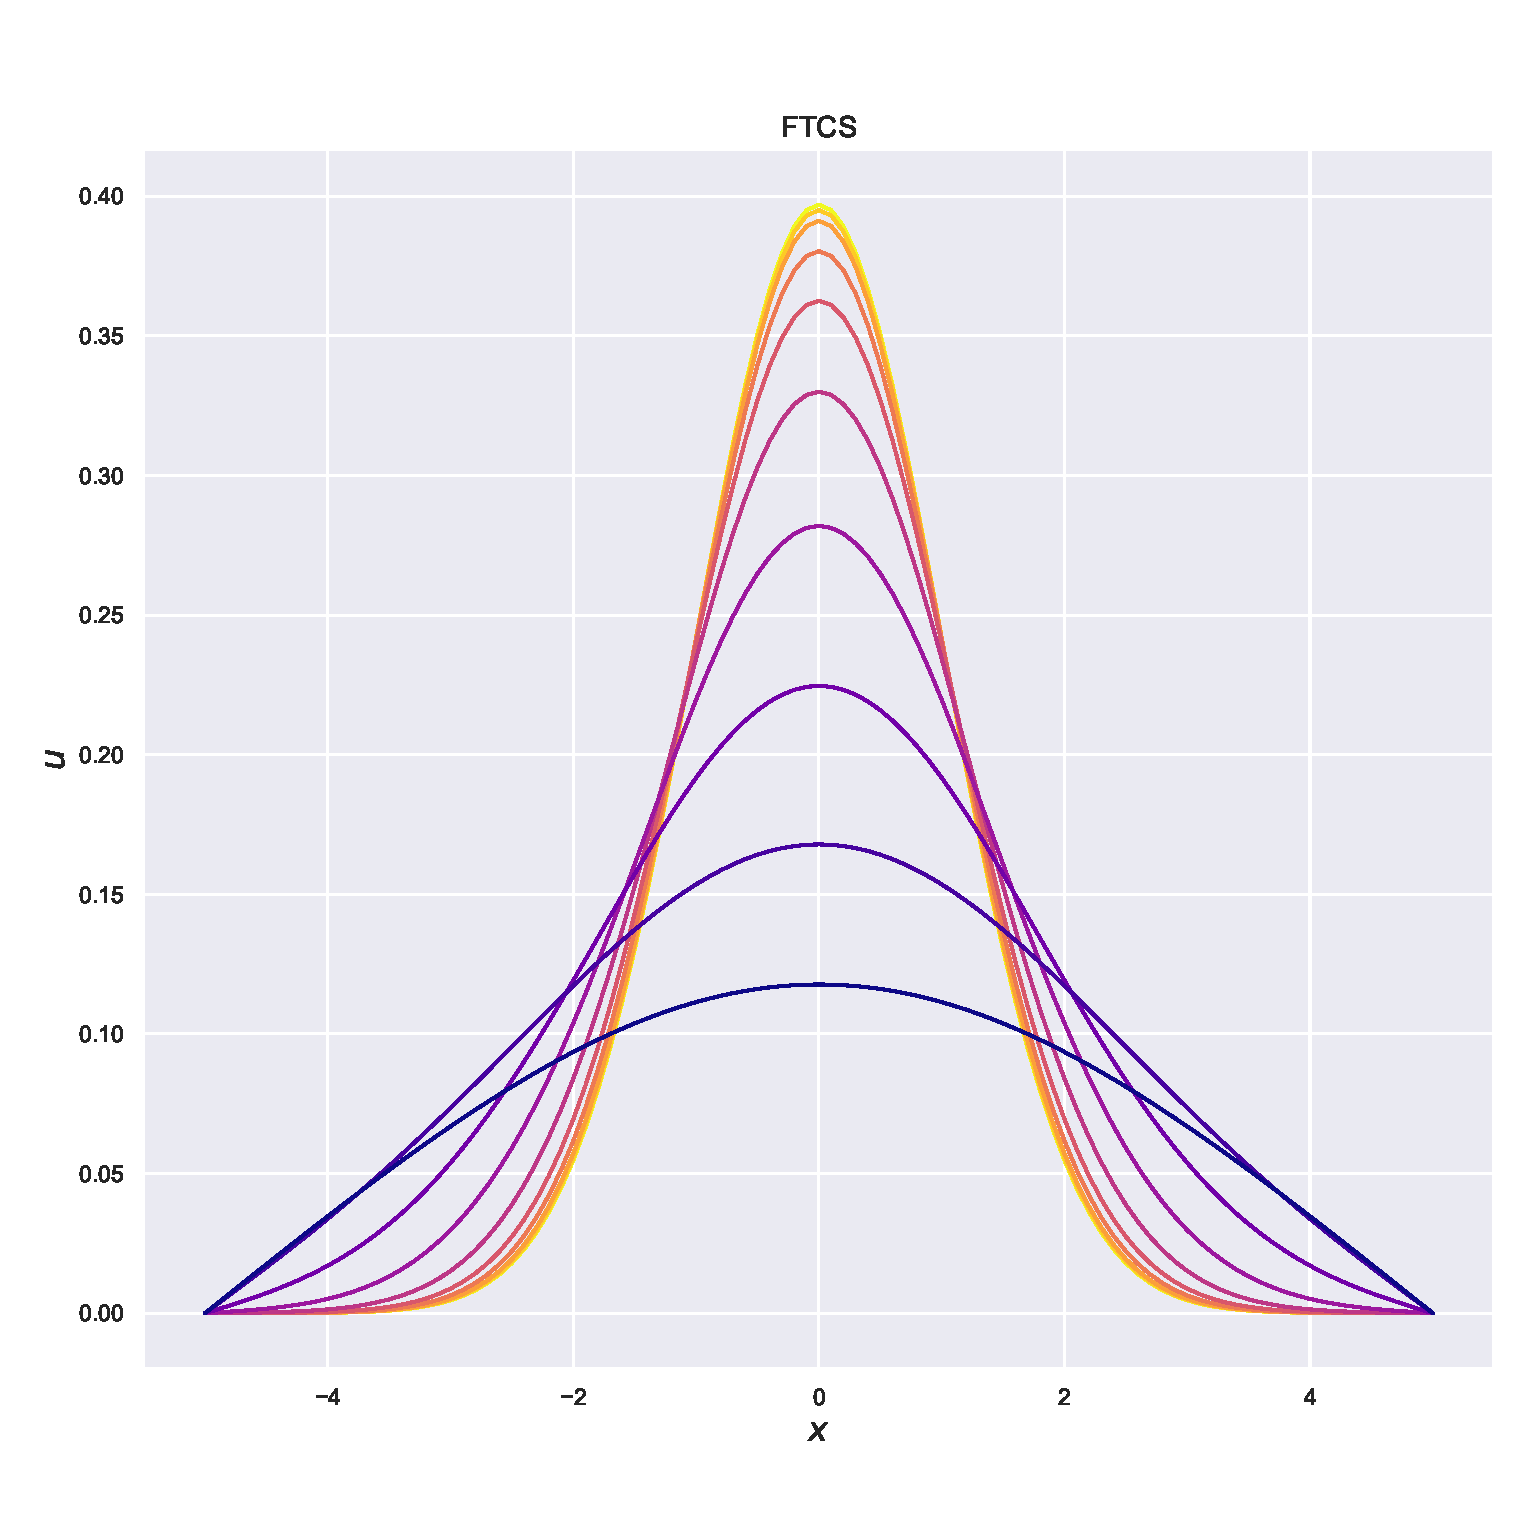
\includegraphics[width=\textwidth]{Figures/stableFTCSheat.eps}
                \subcaption{$\Delta t = 0.005$}
            \end{minipage} %
            \begin{minipage}[b]{0.49\textwidth}
                \centering
                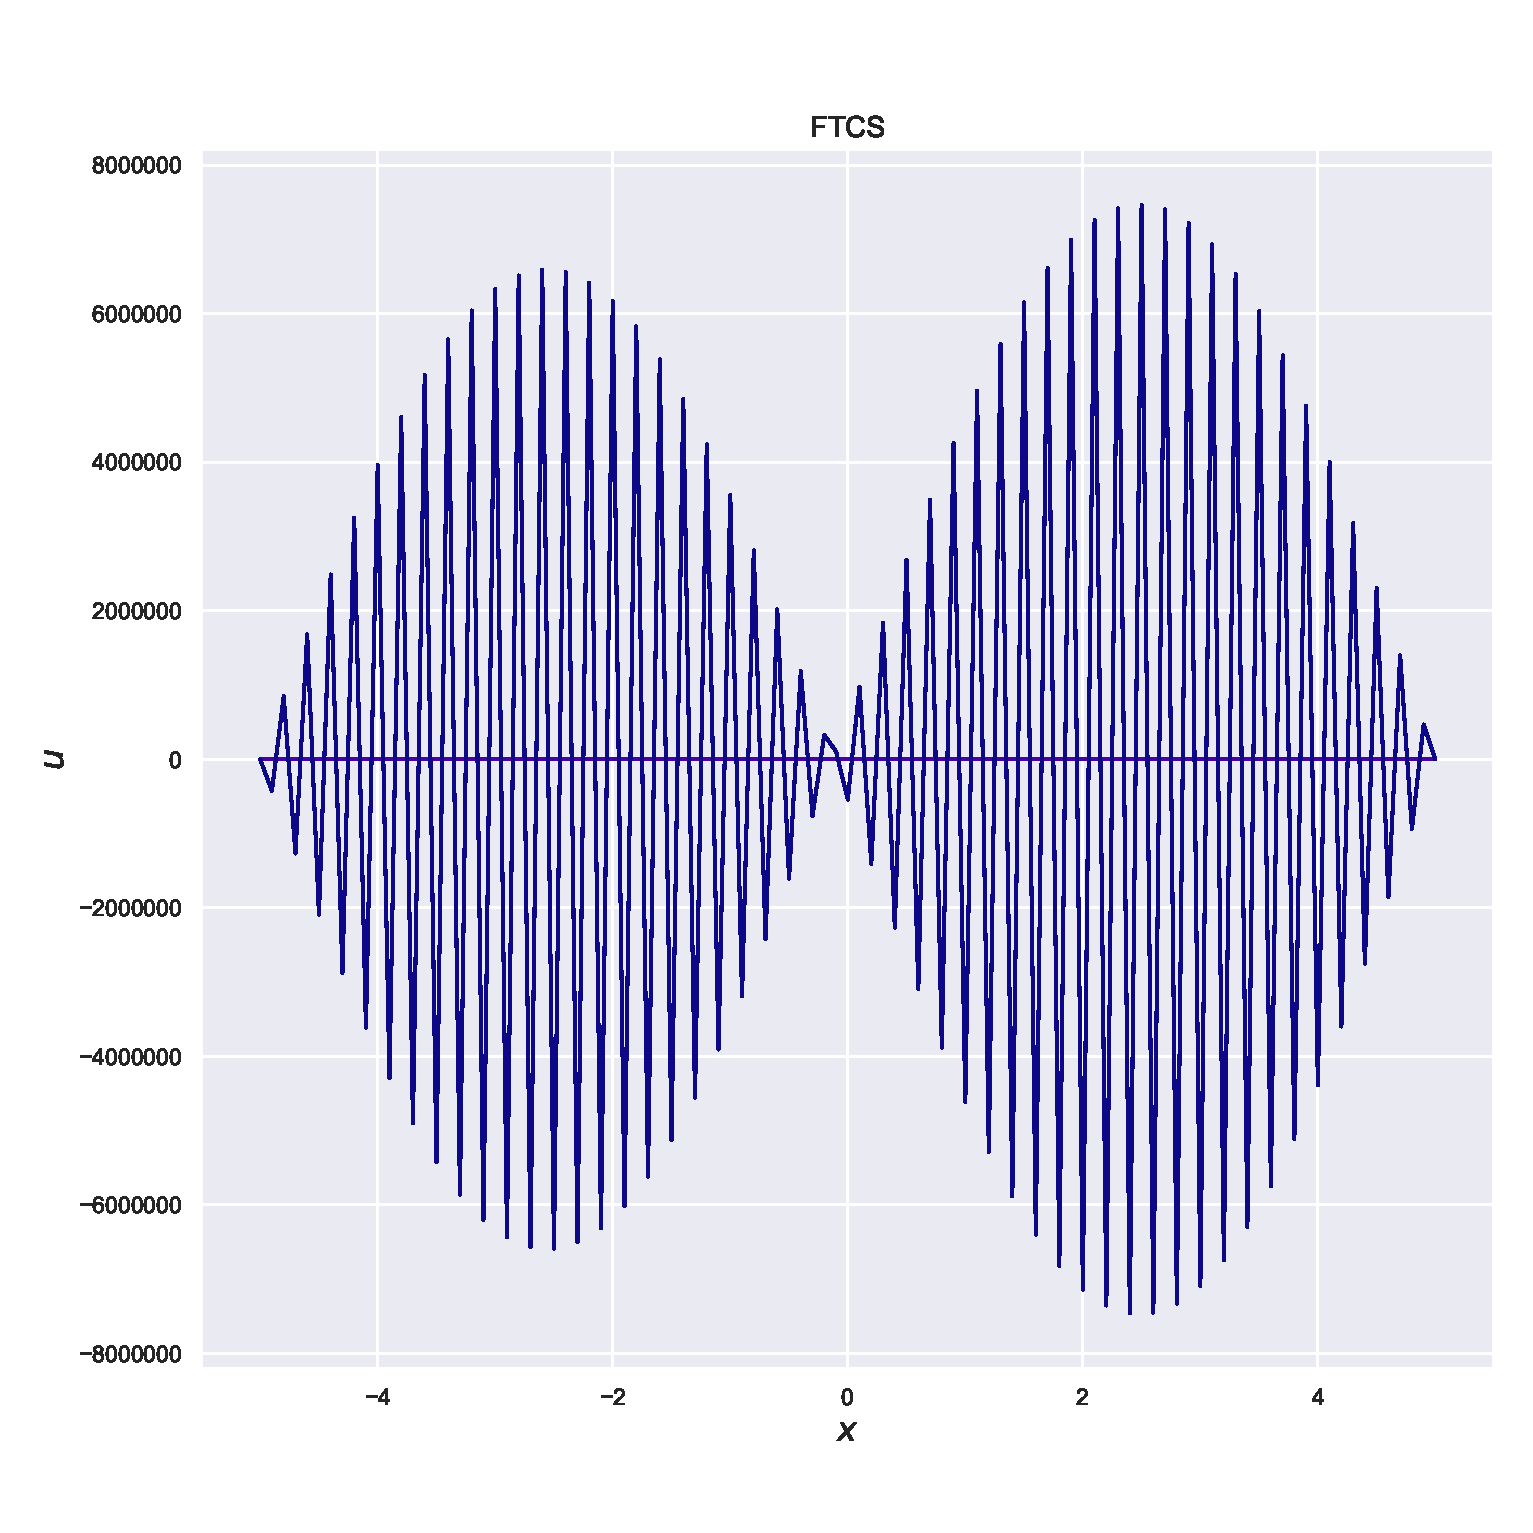
\includegraphics[width=\textwidth]{Figures/unstableFTCSheat.eps}
                \subcaption{$\Delta t = 0.0051$}
            \end{minipage} %
            \caption{Using the \texttt{FTCS} scheme to solve the heat equation \eqref{eq:heat} on $ \lbrack -5,5\rbrack \times\lbrack -1,1\rbrack$ with $\sigma =1, \Delta x = 0.1$ with a Gaussian initial profile.} 
            \label{fig:FTCSunstable}
        \end{figure}
        
        Of these two results, the stability condition is the greater concern. In the next section we look to new methods to remove any restrictions on the mesh spacing, whilst maintaining (or improving) the truncation error.
        
        \subsubsection*{Crank-Nicolson Method}
        To overcome the restriction in mesh spacing, one can use an implicit method, that is one where the solution depends on future time steps as well as the current. A method of this form is not as easy to solve, but as we will show here, has better accuracy and is unconditionally stable. The implicit Euler scheme appears the same as the explicit scheme above however here we calculate the spatial derivative at the future time step in place of the current one as follows:
        \[
          \frac{U^{n+1}_{j}  - U^{n}_{j}}{\Dt} = \sigma \frac{U^{n+1}_{j+1}-2U^{n+1}_{j}+U^{n+1}_{j-1}}{(\Dx)^2}
        \]
        The Crank-Nicolson scheme involves taking the average of the implicit and explicit schemes outlined so far:
        \[
             \frac{U^{n+1}_{j}-U^{n}_{j}}{\Dt} = \frac{\sigma}{2}\left(\frac{U^{n+1}_{j+1}-2U^{n+1}_{j}+U^{n+1}_{j-1}}{(\Dx)^2}+\frac{U^{n}_{j+1}-2U^{n}_{j}+U^{n}_{j-1}}{(\Dx)^2}\right)
        \]
        +++ picture of mesh+++
        Rearranging this equation so that all unknown quantities (future time steps) are on the left hand side gives,
            \[
                -\frac{\mu}{2} U^{n+1}_{j-1} + (1+\mu)U^{n+1}_{j} - \frac{\mu}{2} U^{n+1}_{j-1} = U^{n}_{j} + \frac{\mu}{2} \left( U^{n}_{j+1} - 2U^{n}_{j}+U^{n}_{j-1}\right),
            \]
        where $\mu = \frac{\sigma \Dt}{(\Dx)^2 }$. This is a tridiagonal system and can be reduced to an upper triangular matrix and solved using the Thomas algorithm\footnote{This is also known as the tridiagonal matrix algorithm}. Doing so removes the costly requirement of inverting a matrix.

        As for the stability of such a method, by applying the method seen for the fully-explicit scheme, one obtains 
        \[
            \lambda = \frac{1-2\mu\sin^2\left(\frac{k\Dx}{2}\right)}{1+2\mu\sin^2\left(\frac{k\Dx}{2}\right)}.
        \]
        Here $|\lambda| \not> 1$, so the method is unconditionally stable. We can also apply the same method as before to find the truncation error. Doing so gives that the Crank-Nicolson scheme is second-order in both time and space.
        \begin{figure}
            \centering
            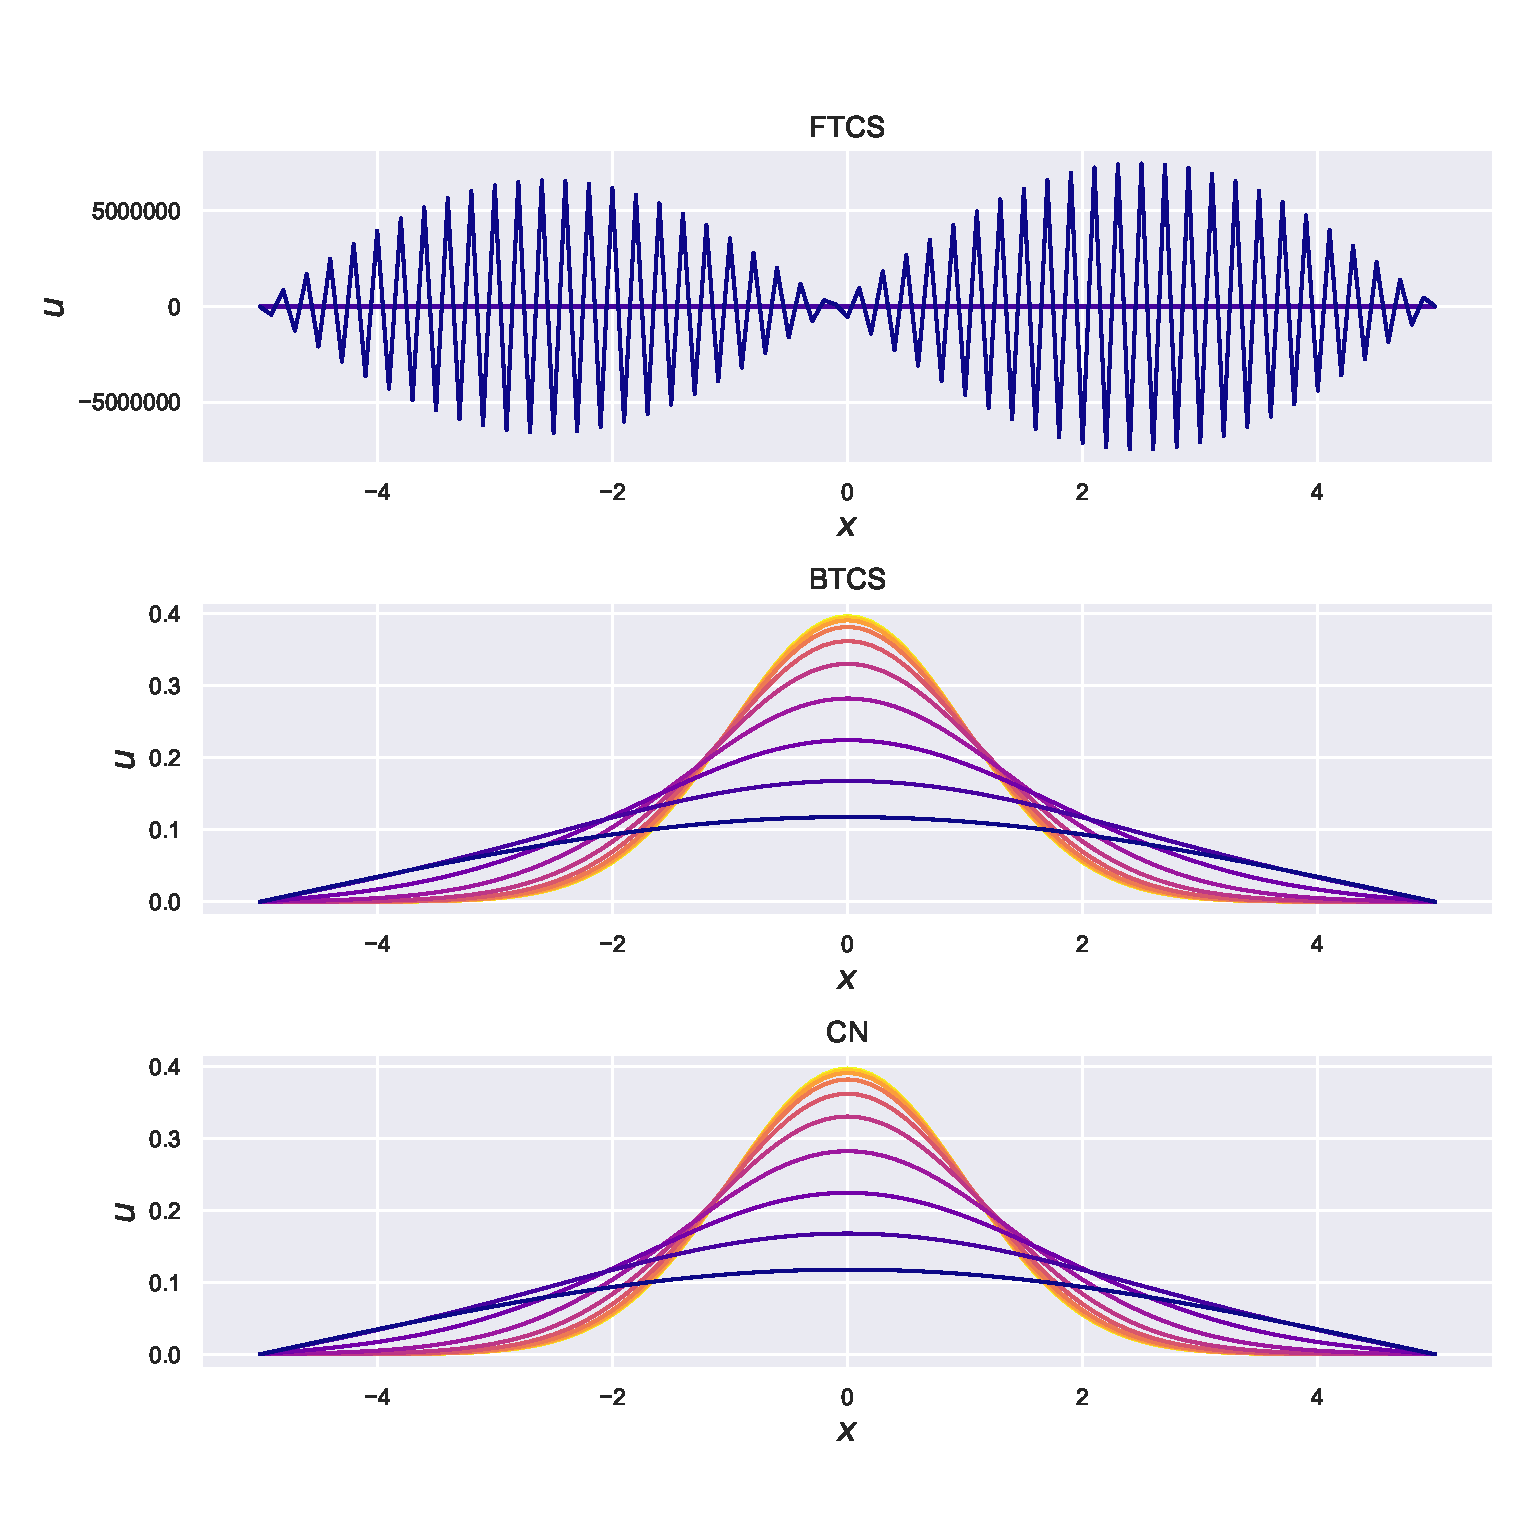
\includegraphics[width=0.7\linewidth]{Figures/FTCSandCN}
            \caption{Solving the heat equation as in Figure \ref{fig:FTCSunstable} using \texttt{FTCS, BTCS} and \texttt{CN} respectively. The implicit solvers remain stable regardless of step size.}
            \label{fig:ftcsandcn}
        \end{figure}
        
        \subsection{Advection Equations}
        Our prototypical example in this case will be the one-way wave equation,
        \begin{equation}\begin{cases}
            \partial_t u(t,x) + a\partial_x u(t,x)=0,\\
            u(0,x) = u_0(x),  &t\in\R^+, x\in\R.
        \end{cases}\label{eq:wave}\end{equation}
        Using the same discretisation as for the time derivative in the diffusion equation, yields the first order upwind scheme,
        \[
            \frac{U^{n+1}_{j}-U^{n}_{j}}{\Dt} = \begin{cases} a\frac{U^{n}_{j+1}-U^{n}_{j}}{\Dx} & \text{ if } a>0\\[0.5em]
                                                              a\frac{U^{n}_{j}-U^{n}_{j-1}}{\Dx} & \text{ if } a<0\\
                                                \end{cases}
        \]
        If the sign of \(a\) is not taken into account, the scheme is unstable. For further details see \cite{Hundsdorfer2007}.
        +++Error, modified equation showing dispersion +++
        
        \begin{figure}
            \centering
            \begin{minipage}[b]{0.49\textwidth}
                \centering
                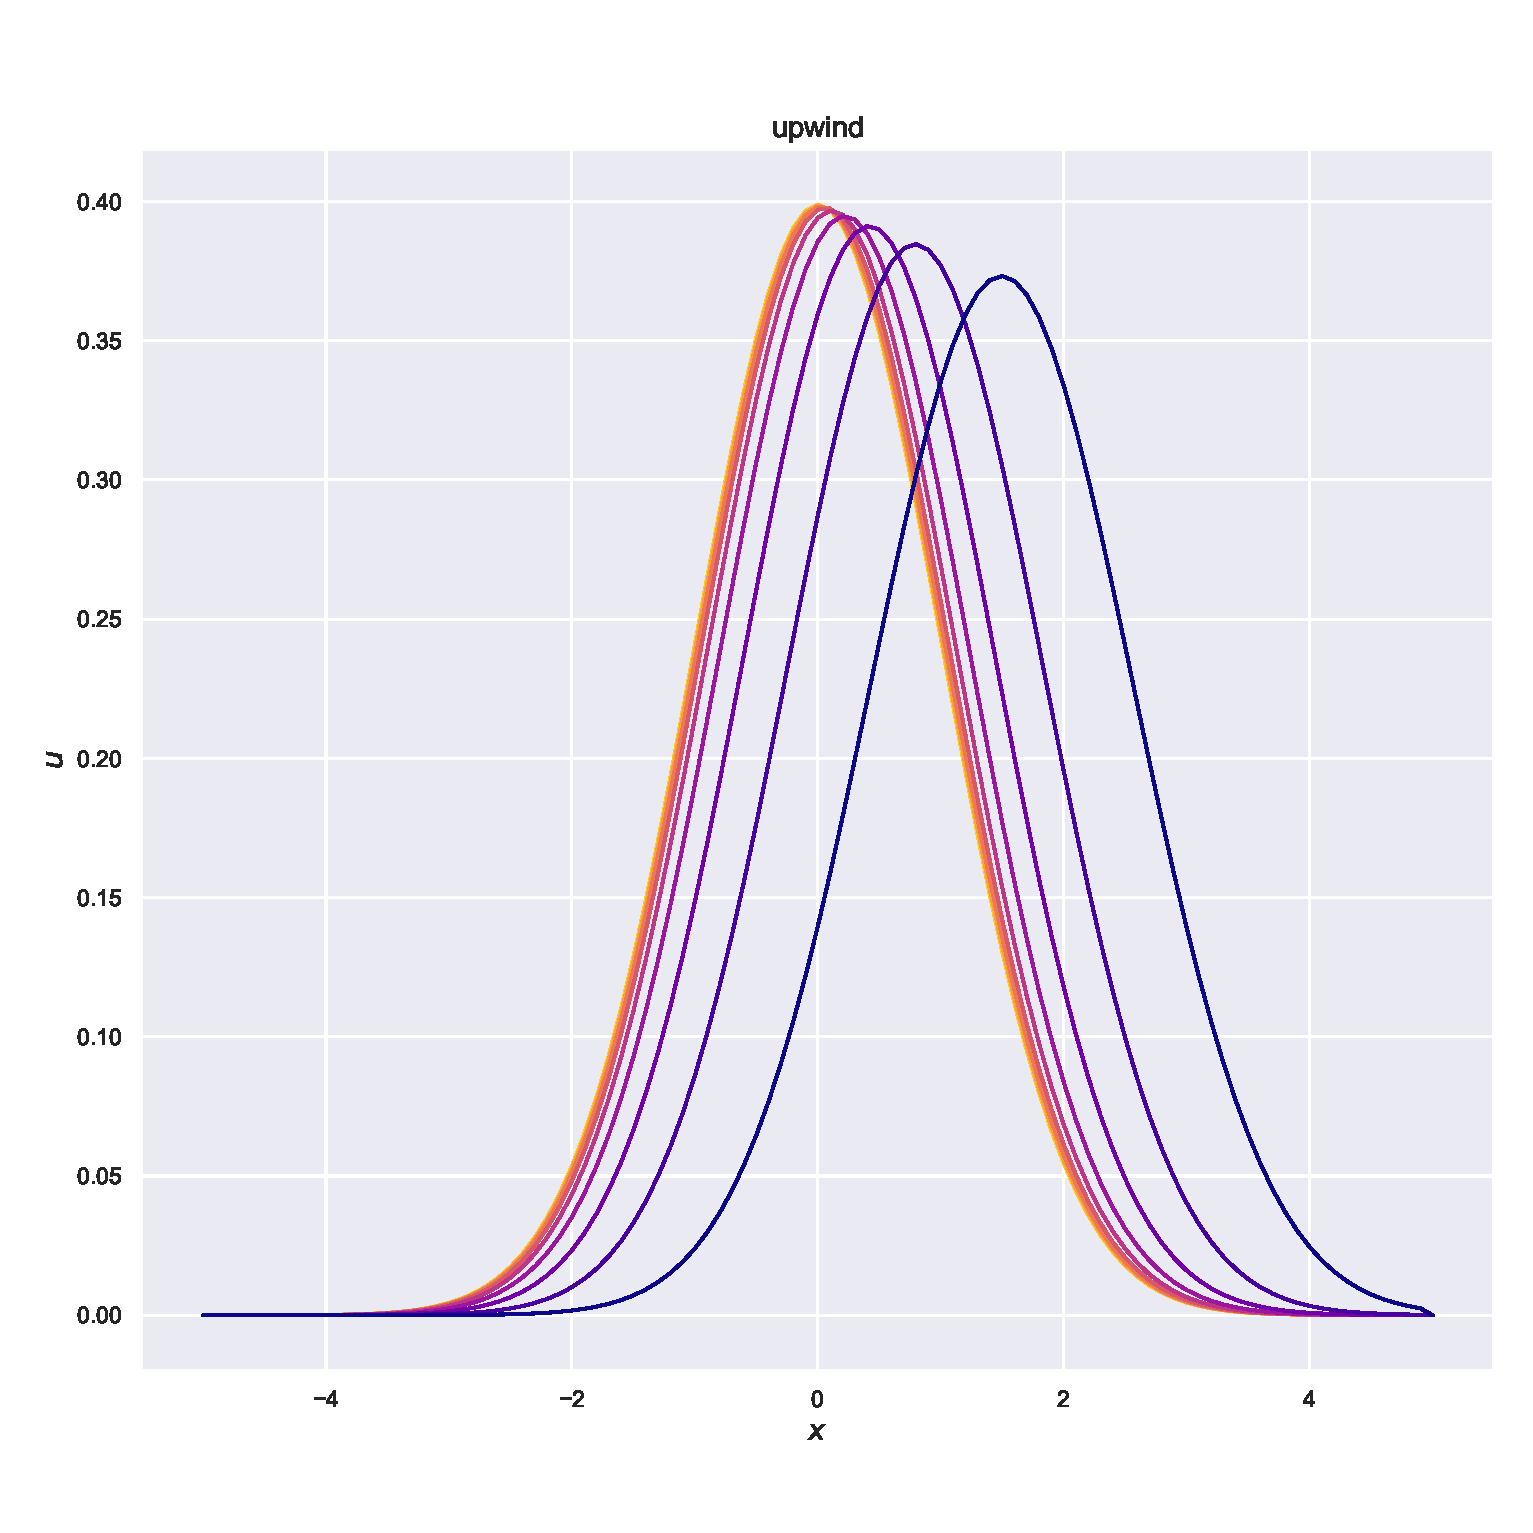
\includegraphics[width=\textwidth]{Figures/advgaussian.eps}
                \subcaption{$U_0 \sim \mathcal{N}(0,1)$}
            \end{minipage} %
            \begin{minipage}[b]{0.49\textwidth}
                \centering
                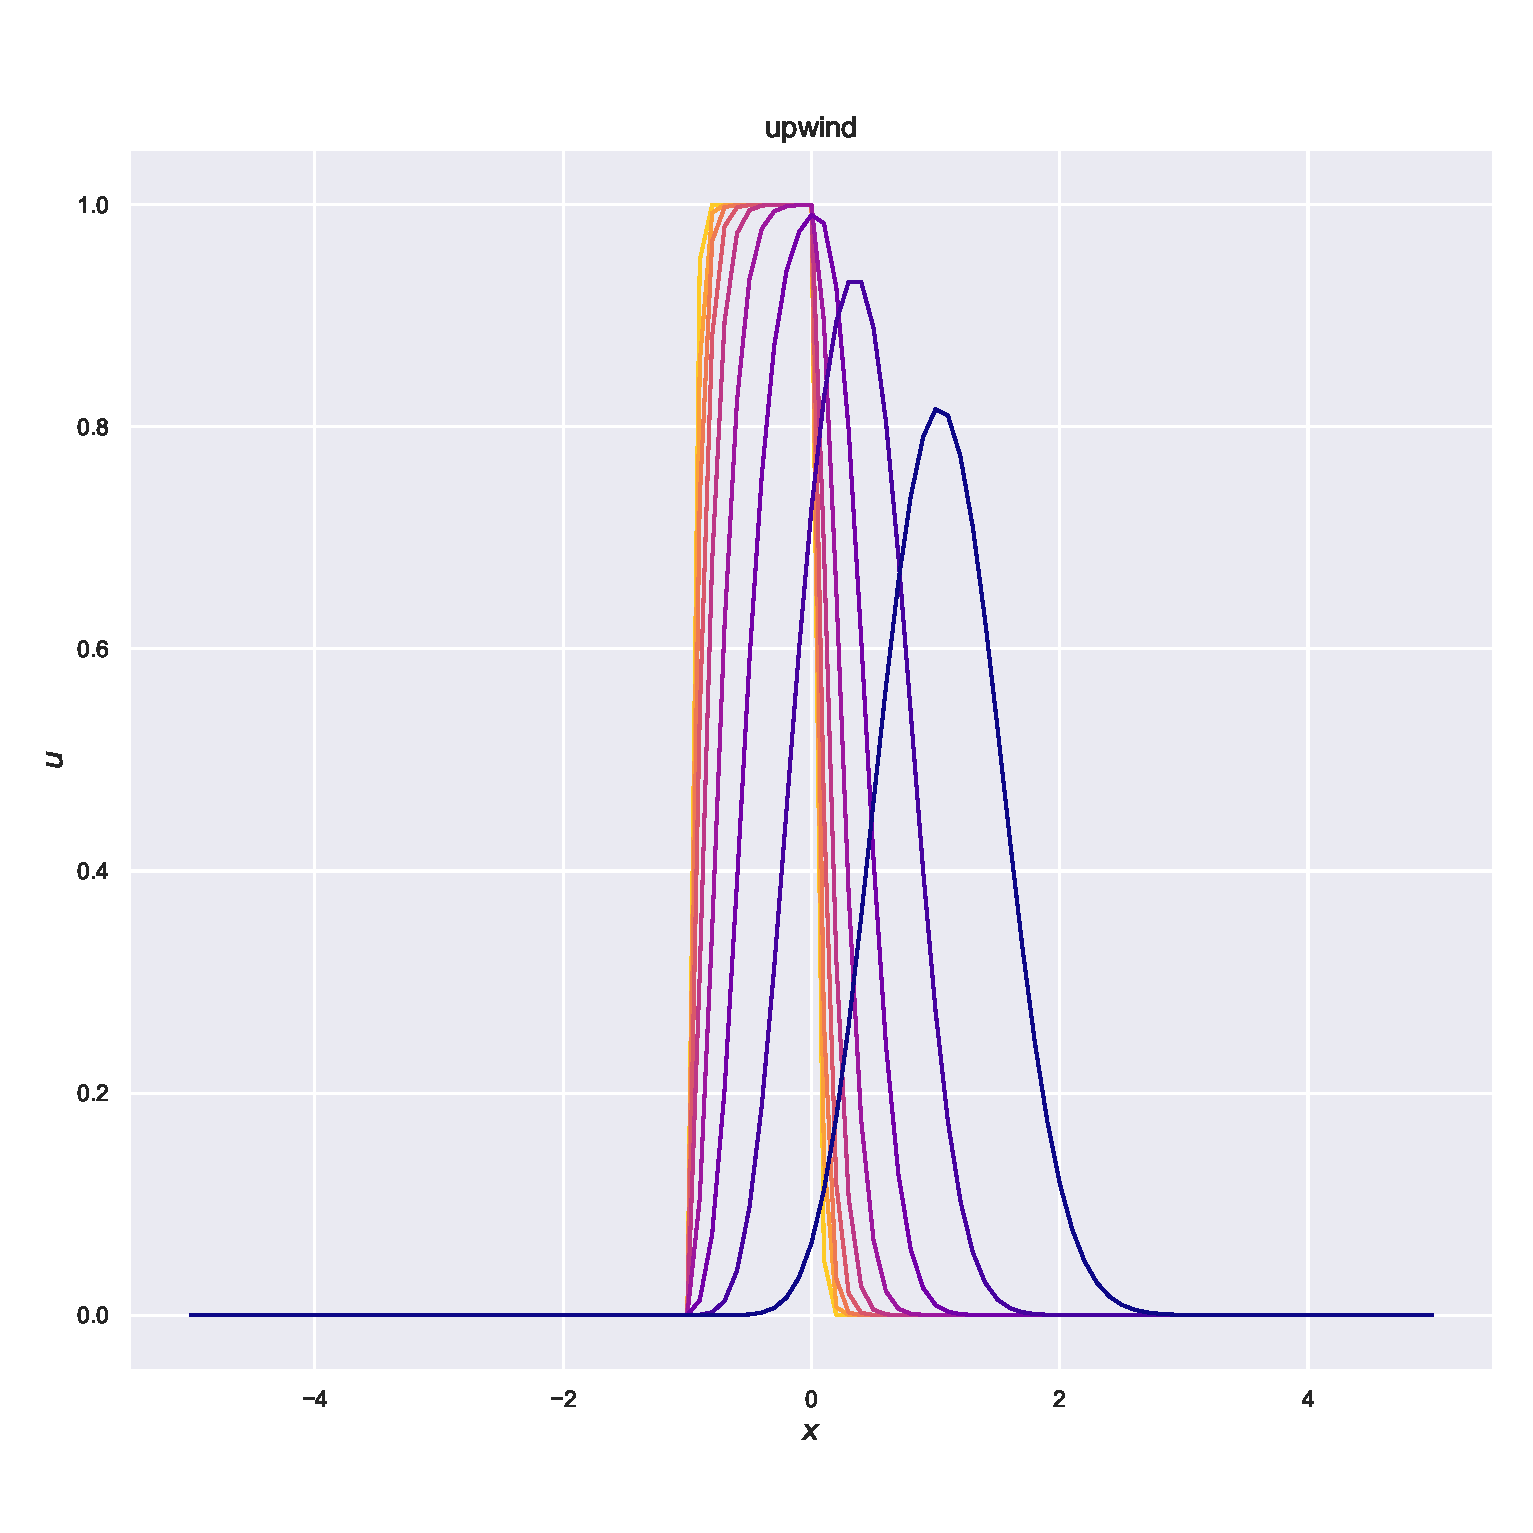
\includegraphics[width=\textwidth]{Figures/advindicator.eps}
                \subcaption{$U_0(x) = \mathbbm{1}_{\lbrack-1,0\rbrack}(x)$}
            \end{minipage} %
            \label{fig:advection}
            \caption{Solving equation \eqref{eq:wave} with the upwind scheme. Even with very smooth initial data, dispersive effects can be severe.} 
        \end{figure}
    
        \subsection{Finite Volume Schemes}
        In Section \ref{sec:dynamics}, equations were closed on the moments of the distribution. From this, we know that \(\dot{M}_0 = 0\), that is mass is conserved. This suggests that numerical schemes designed to conserve mass would be ideal for solving this system. One such method is a finite volume scheme, a generalisation of finite difference methods. First, we write the system in conservative form. This is an equation of the form $\partial_ u = \partial_x(a(x)u)$. For the space homogenous model \eqref{eq:space_hom_PDE}, this corresponds to
        \begin{equation}\label{eq:flux_space_hom}
        \partial_t f_t = \partial_v \left[\left(v-G(\langle w \rangle_{f_t})\right)f_t + \sigma \partial_v f_t \right].
        \end{equation}
        Using the same discretisation as in Section \ref{sec:numericalmethods}, we further introduce auxiliary points $v_{j\pm\frac{1}{2}} = \frac{1}{2}(v_{j\pm1} + v_j) $. Then within any cell (or volume), $\Omega_j = [v_{j-\frac{1}{2}}, v_{j+\frac{1}{2}}]$, we can calculate the average.
        \[
        \bar{f}_t(v_j) = \frac{1}{\Dv}\int_{\Omega_j} f_t(v) \dif v = f_t(v_j)+\frac{1}{24(\Dv)^2} \partial_{vv} f_t(v_j)
        \]
        Furthermore, the change in the average density within the cell is equal to difference of the mass lost through either side of the volume, that is,
        \[
        \Dv\od{\bar{f}_t(v_j)}{t} = a(v_{j-\frac{1}{2}})f_t(v_{j-\frac{1}{2}}) - a(v_{j-\frac{1}{2}})f_t(v_{j-\frac{1}{2}}), 
        \]
        where $a(v) = \left[\left(v-G(\langle w \rangle_{f_t(v)})\right)f_t + \sigma \partial_v f_t(v) \right]$. This can then be approximated using a finite volume scheme:
        \[
        \frac{F^{n+1}_j - F^n_j}{\Dt} = \frac{1}{\Dv}\left[ a(v_{j-\frac{1}{2}})F^n_{j-\frac{1}{2}} - a(v_{j-\frac{1}{2}})F^n_{j-\frac{1}{2}}\right]
        \]
        This is the first-order upwind scheme in conservative (flux) form. As in the previous upwind scheme, the choice of spatial points at which to evaluate depends on the sign of the advection term. That is,
        \[
        a(v_{j+\frac{1}{2}})F^n_{j+\frac{1}{2}} = a^+(v_{j+\frac{1}{2}})F^n_{j} + a^-(v_{j+\frac{1}{2}})F^n_{j+1},
        \]
        where $a^+ = \max(a,0), a^- = \min(a,0)$.  This scheme is still order 1, however it provides the ideal setting for developing higher order schemes.
        +++show agreement with FD, particle,  show symmetry in error+++ 
        
          
		\section{Applying the Numerical Scheme}
			We now have enough techniques to begin solving the kinetic model. Consider the space-homogeneous evolution given by \eqref{eq:space_hom_PDE}, that is
			\begin{equation}
				\partial_t f_t(v) = \partial_v vf_t(v) - \partial_v G(\langle w \rangle_{f_t})f_t(v) + \sigma \partial_{vv} f_t(v).
			\end{equation}
            Using the methods developed in the previous section, we are now able to solve this system numerically. As when solving the heat equation, a zero boundary condition shall be enforced. This is valid as we know that the stationary distributions are Gaussian and centred at $-1,0,+1$. The boundary $L$ can then be chosen depending on the the diffusion so that almost no mass is contained beyond the boundary. For example if $\sigma = 1$, the mass contained beyond $L=5$ is of the order $10^{-5}$. 
            
			Simpson's rule will be used as a quick way to approximate the integral within the herding coefficient. To differentiate between the integral and its approximation, we write \(\langle w\rangle_{F^n}\). Below is the scheme when both the herding coefficient and the velocity are positive, using a finite difference scheme with a CN discretisation for the diffusive term and an upwind method for the damping and herding terms.
			\begin{equation*}
			\begin{split}
				\frac{F_j^{n+1} - F_j^n}{\Delta t} = 	-G(\langle w\rangle_{F^n})\left[ \frac{F^n_{j+1} - F^n_{j}}{\Delta v}\right] &+\left[ \frac{v_{j}F^n_{j} - v_{j-1}F^n_{j-1}}{\Delta v}\right]\\ &+ \frac{\sigma}{2}\left[ \frac{F^{n+1}_{j+1} - 2F^{n+1}_j + F^{n+1}_{j-1}}{(\Delta v)^2} + \frac{F^{n}_{j+1} - 2F^{n}_j + F^{n}_{j-1}}{(\Delta v)^2}\right] 	 
			\end{split}
			\end{equation*}

			+++Pictures, moments converging, error (in moments too?) in particular, mass loss? -> compare conservative methods i.e. fin vol +++
   \subsection{Space Heterogeneous}
        +++ phi = 1 still, moving in space. Animations/diagrams showing Leb in space. +++
        
        \section{Discussion + Conclusion}
        +++ future add other phi, recalc M +++
	\bibliographystyle{abbrv}
	\bibliography{whales.bib}
	\appendix

\end{document}